% This is samplepaper.tex, a sample chapter demonstrating the
% LLNCS macro package for Springer Computer Science proceedings;
% Version 2.21 of 2022/01/12
%
\documentclass[runningheads]{llncs}
%

%
\usepackage[T1]{fontenc}
\usepackage{comment}
% T1 fonts will be used to generate the final print and online PDFs,
% so please use T1 fonts in your manuscript whenever possible.
% Other font encondings may result in incorrect characters.
%
\usepackage{graphicx}
\usepackage{enumitem}
\usepackage{amssymb}
% Used for displaying a sample figure. If possible, figure files should
% be included in EPS format.
%
% If you use the hyperref package, please uncomment the following two lines
% to display URLs in blue roman font according to Springer's eBook style:
%\usepackage{color}
%\renewcommand\UrlFont{\color{blue}\rmfamily}
%\urlstyle{rm}
%
\begin{document}
%\bibliographystyle{splncs04}
%\bibliography{LLMs and Data Streams}
%
\title{Large Language Models and Data Streams}
%
%\titlerunning{Abbreviated paper title}
% If the paper title is too long for the running head, you can set
% an abbreviated paper title here
%
\author{Silyu Li}
%
%\authorrunning{F. Author et al.}
% First names are abbreviated in the running head.
% If there are more than two authors, 'et al.' is used.
%
\institute{RWTH Aachen University, Aachen, Germany
%\email{lncs@springer.com}\\
%\url{http://www.springer.com/gp/computer-science/lncs} \and
%ABC Institute, Rupert-Karls-University Heidelberg, Heidelberg, Germany\\
%\email{\{abc,lncs\}@uni-heidelberg.de}
}
%
\maketitle              % typeset the header of the contribution
%
\begin{abstract}
    Large language models, such as ChatGPT, have become widely recognized and are extensively utilized across various domains. However, these models are typically trained on static datasets, lacking updates to new data beyond their initial training set. 
    To enable models that can continuously update themselves based on incoming data, it is necessary to have large language models trained and updated on input data streams.

    In this paper, we begin by outlining the structure and fundamental applications of large language models. Subsequently, we introduce the concept of data streams and provide an overview of current use cases where large language models are adapted to accommodate streaming data. Finally, we summarize the existing challenges associated with integrating large language models with data streams and discuss potential solutions.
\keywords{LLM  \and data streams \and chatGPT.}
\end{abstract}
%
%
%
\section{Introduction}
Large language models have shown their wide usage and significant competence in many fields according to \cite{Liu23}, such as learning and answering users' questions in academic fields,
assisting in diagnosing diseases in medical fields, generating text and classifying text data to various categories etc. However, as \cite{Gupta23} demonstrates, 
there is a significant limitation of current large language models: they are trained based on certain static datasets that will not automatically be updated, and this causes the resulting models to only be able to access information from its training datasets. 
When the models need to be updated as new data becomes available, the only way is to start the training process over again. But in many scenarios such models can't satisfy our needs. 
For example, to have a better traffic prediction, real-time traffic data is needed \cite{Zhang24},
Analyzing news and events sentiment can help predict the financial market \cite{Araci19}, 
real-time health data is of great importance when monitoring patients' health condition \cite{Thiru23} etc.
So to have models that can fulfill those use cases, we need to find and compare useful methods that combine large language models and continuous data input (data streams) together, and also summarize the current major obstacles. 

\section{Related Works}
In this chapter, the following concepts and techniques that are related to this topic will be covered.

\subsection{Large Language Model}
In this subsection, I will talk about the following aspects of large language models:
    
  
\subsubsection{The evolution of large language models}  
\noindent \newline 
The earliest language models, taking n-grams as an example, are statistical. n-grams refers to an N-characters substring of a longer string and n represents the length of the substring, according to \cite{Cavnar94}.
Taking the sentence "I read a book" as example, a bi-grams composition of this sentence would be "I read", "read a" and "a book". By considering the n previous words, the frequency and probability of each
n-grams can be calculated, which makes n-grams model perform well in text classification and word prediction with short documents \cite{Cavnar94}. 
However, n-grams performs poorly with long documents due to the rapid growth of dimensionality with large n, and it has only restricted access to the words that appear in the document.\\
\noindent \newline
Later models using word embeddings such as Word2Vec solve the problems of earlier models to some extent by representing words in vector spaces, and words with similar meanings such as "walk" and "run" have closer distance
in the vector space \cite{Mikolov13}. Word embeddings successfully reduces the dimensionality of word representations and can work with larger documents by combining techniques such as "Continuous Bags of Words" \cite{Mikolov13}. \\   
\noindent \newline
With the development of neural networks, more powerful models such as the Seq2Seq model began to take a more important role in many application fields such aspects
machine translation \cite{Sutskever14}. The core idea of the Seq2Seq model is that it uses the Long Short-Term Memory networks as an encoder to map the input to a vector with fixed dimensionality, and then
uses another LSTM to decode the output sentence from the vector. The use of LSTM makes it possible for the model to handle long input sequences and the encoder-decoder structure enables the model 
to manage different lengths for input and output sequences \cite{Sutskever14}. \\
\noindent \newline
Large language models start to have a huge leap forward after the introduction of the transformer architecture \cite{Vaswani17}. \cite{Radford18} demonstrates that the transformer architecture can
effectively improve the language understanding ability of language models even with large unlabeled text corpora by first generatively pre-training the model on the text data and then discriminative fine-tuning them on various tasks.
According to \cite{Radford19}, large language models such as GPT-2 (with 1,5 billion parameters) are trained on massive training datasets including the crawling results from millions of different web pages, called WebText.
As for the relationship between model performance, the number of model parameters $N$, the size of dataset $D$ and the amount of computing to train the model $C$, \cite{Kaplan20} demonstrates the \textbf{Smooth Power Laws} which says:
"Performance has a power-law relationship with each of the three scale factors N, D, C when not bottlenecked by the other two, with trends spanning more than six orders of magnitude". Nowadays, there are various models
that have distinct capabilities, for example, DALL-E can generate and modify images based on text input, whereas ChatGPT 3.5 can generate code and natural language \cite{Gozalo23}.
\noindent \newline
\begin{figure}[]
  \centering
  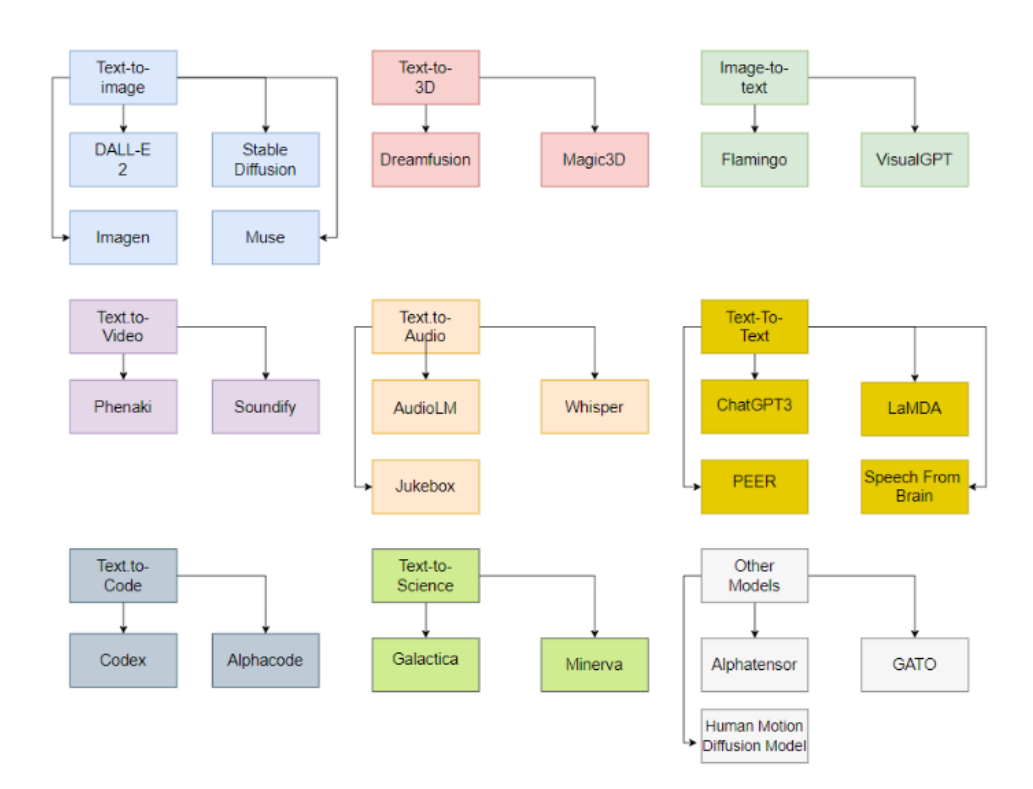
\includegraphics[width=0.7\textwidth]{models overview.png}
  \caption{An overview of the recent major generative AI models  \cite{Gozalo23}}
  \label{fig:model_overview}
\end{figure}

\subsubsection{The architecture and training process of large language models}
\noindent \newline
As discussed before, large language models such as ChatGPT and BERT are based on transformer-based neural networks. The transformer architecture, as figure \ref{fig:attention} shows, is an 
encoder-decoder architecture. According to \cite{Vaswani17}, the encoder takes the input sequence and converts them into dense vectors of fixed size at the input embedding step. Then with the 
help of the positional encoding step, the input sequence contains information about each token in the sequence. The encoded inputs are then passed through the multi-head attention mechanism so that the 
model can capture various relationships and features from the input sequence. Then the Add and Normalization layer is applied to stabilize and speed up the training process. In the end, the Feed Forward layer is 
applied to help in introducing non-linearity and learning complex representations for each token's position in the sequence. Similarly, the decoder uses the vector representation of the input sequence created
by the encoder along with the previously generated tokens to produce the next token in the output sequence and the masked multi-head attention mechanism is applied to ensure that the prediction for a particular position depends only on the known outputs at earlier positions. \\
\noindent \newline
Various input text datasets must be pre-processed before they can be used for the training process, and the data pre-processing includes the following steps \cite{Roum23}:
\begin{itemize}
  \item Tokenization involves segmenting text into tokens, which are the basic units of broken text. Tokenization can simplify and standardize the input data and improve model performance \cite{Devlin18}.
  \item Subword encoding refers to breaking down the input text into smaller units and helping handle rare or out-of-vocabulary words in the input text.
  \item Data cleaning is the step where the noisy information in the input data should be removed, which can significantly improve the quality and suitability of the input data for the model.
\end{itemize} 
\noindent \newline
The model starts its training algorithm after taking the pre-processed data as its input. For models such as ChatGPT and BERT, their training algorithm consists of an unsupervised pre-training phase and a supervised fine-tuning phase \cite{Roum23}.
In the pre-training phase, a large amount of unlabeled WebText data is used as the model's training dataset to make it a high-capacity language model. Given an unlabeled corpus of tokens $U=\{u_1,...,u_n\}$ as training dataset, the core idea of the pre-training phase is to 
predict the next token $u_i$ for a sequence $\{u_{i-k},...,u_{i-1}\}$. According to \cite{Radford18}, this is done by maximizing the likelihood: 
\begin{equation}
  L_1(U) = \sum_{i}\log{P(u_i|u_{i-k},...,u_{i-1}; \Theta)}
\end{equation}
$k$ refers to the context window size and $\Theta$ is the parameter of the neural network with which the conditional probability $P$ is modeled. \\
\noindent \newline
The supervised fine-tuning phase is used to improve the model's performance on specific tasks by training it on a smaller corpus of labeled data \cite{Roum23}. Given a labeled dataset $C$,
where each instance of $C$ has a sequence of tokens \{$c^1,...,c^m$\} and a label $y$, the goal of the fine-tuning phase is to maximize the following likelihood \cite{Radford18}:
\begin{equation}
  L_2(U) = \sum_{(x,y)}\log{P(y|x^1,...,x^m)}
\end{equation}

  \begin{figure}[htbp]
      \centering
      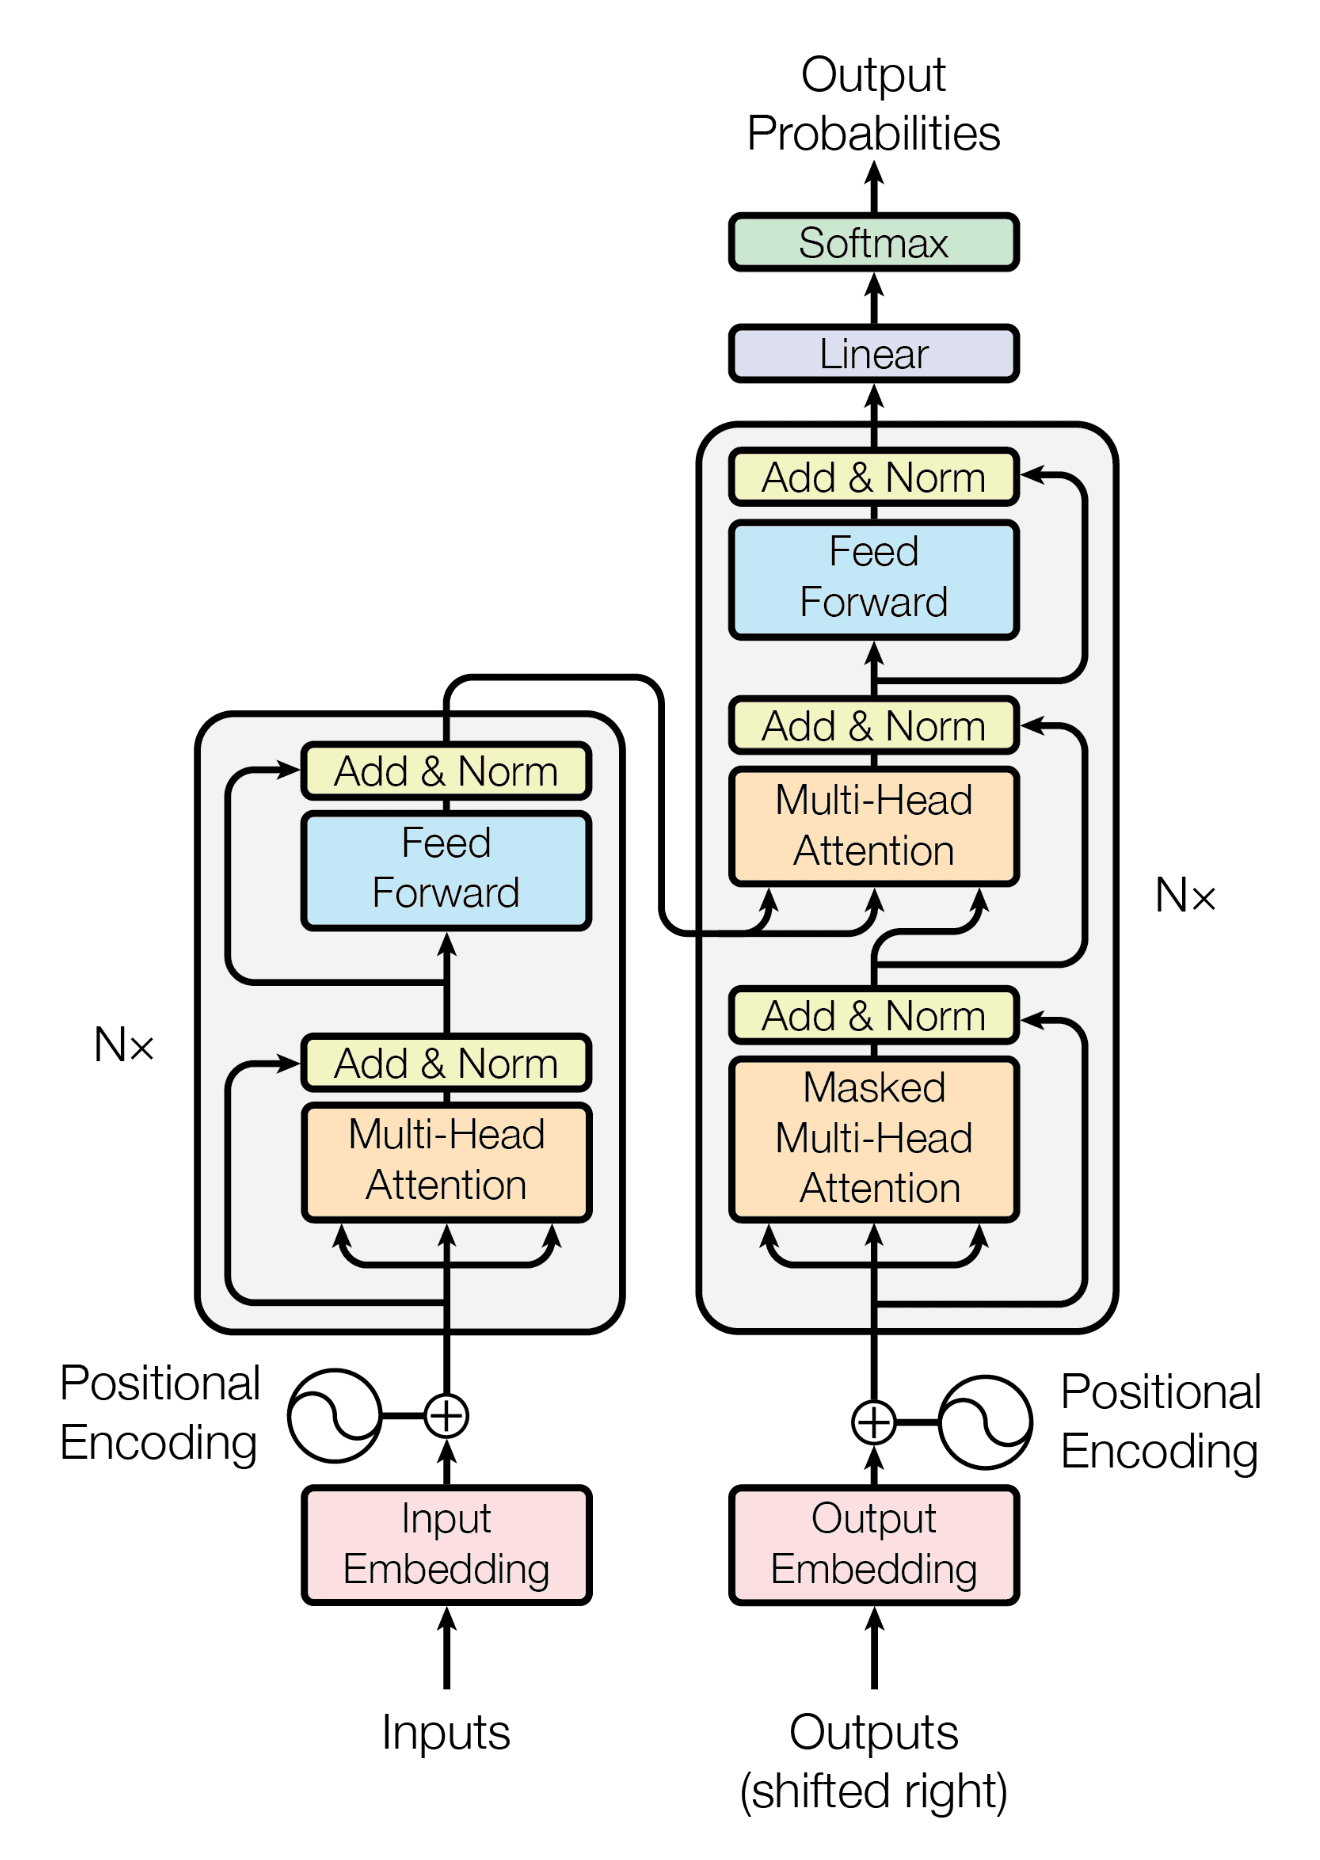
\includegraphics[width=0.6\textwidth]{attention1.jpg}
      \caption{The transformer structure \cite{Vaswani17}}
      \label{fig:attention}
  \end{figure}

%\begin{figure}[]
%    \centering
%    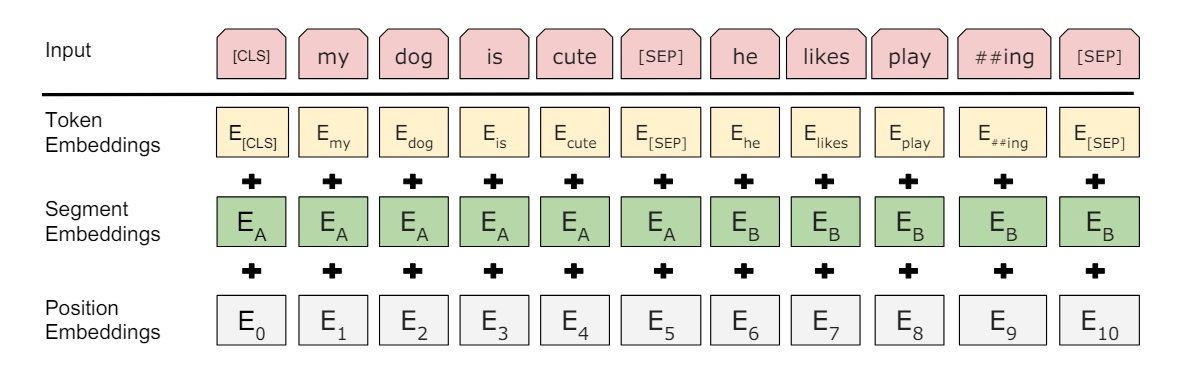
\includegraphics[width=0.7\textwidth]{BERT input repres.png}
%    \caption{Input representation in the BERT model \cite{Devlin18}}
%    \label{fig:bert_input}
%\end{figure}

\subsection{Data Stream}
Data stream has many informal definitions, \cite{Patro06} describes data stream as "time-varying, volatile, unpredicted and possibly unbounded information". \cite{Golab03} describes data stream as
"a data set that is produced incrementally over time, rather than being available in full before its processing begins". According to \cite{Geisler13}, data stream has the following formal definition:
\begin{definition}
  A data stream $S$ is an unbounded, potentially infinite multiset of data stream elements $(s,\tau)$, where $\tau \in \mathbb{T}$. $\mathbb{T}$ is a timestamp attribute with values from a monotonic, infinite time domain $\mathbb{T}$ with discrete time units.
\end{definition}


\subsubsection{The definition of data streams} With the definition from different sources \cite{Geisler13}.

\subsubsection{The use case of data streams} Data streams are the key components in many application fields such as Weather Forecasting, Health monitoring, Internet of Things etc \cite{Geisler16}.

\section{Use Cases and Obstacles}
In this section, I will give an overview of current use cases where large language models and data streams are combined, and also summarize the major challenges of combining large language models with data streams. Furthermore I will also give an introduction of what measurements have been taken to mitigate the obstacles. 
\subsection{Use Cases}
Following use cases will be covered:
\begin{itemize}
    \item Social Media Monitoring: Analyzing streaming data from social media platforms can help monitor regional news, sentiment, and trends in real-time.
    \item Financial Monitoring:  Large language models can analyze streaming news feeds to identify important events, trends, and sentiment in real-time. This can be valuable for financial institutions and risk management companies to stay informed about current events and market trends.
    \item Health Care Monitoring: Large language models can analyze streaming medical data such as patient records, diagnostic reports, and research papers to assist healthcare providers in diagnosing diseases, identifying treatment options, and monitoring public health trends in real-time.
    \item Traffic Data Monitoring: Large language models can analyze streaming traffic data to monitor traffic conditions in real-time to help reduce traffic accidents and level up transportation efficiency. 
    %\item Security and Threats Detection: Large language models can analyze streaming data from network logs, security alerts, and threat intelligence feeds to detect and respond to cybersecurity threats in real-time. This includes identifying suspicious activities, malware signatures, and potential vulnerabilities.
\end{itemize}
\begin{figure}[]
  \centering
  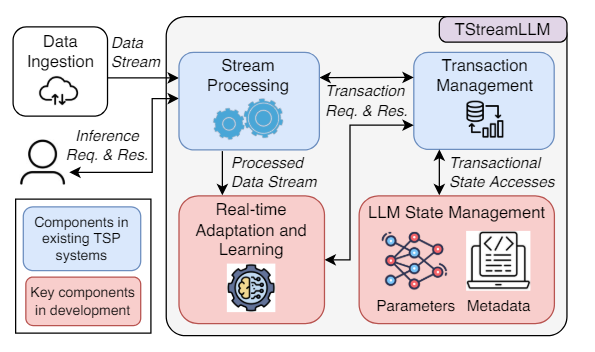
\includegraphics[width=0.7\textwidth]{TStreamLLM architecture.png}
  \caption{Architecture of TStreamLLM \cite{Zhang24}}
  \label{fig:TStreamLLM}
\end{figure}

\subsection{Comparison of LLMs with static datasets and data streams}

\subsection{Challenges}
Following challenges will be covered:
\begin{itemize}
    \item Catastrophic forgetting \cite{Gupta23}
    \item Concept drift: if the LLM is trained for a long time, it is possible that the relationship between the inputs and the outputs itself might change.
    \item Computational resources: continuous learning requires significant computational resources, which may be costly or impractical to scale.
    \item Privacy and security:  streaming data often contains sensitive or private information, raising concerns about data privacy and security.
    \item Data quality: data streams may contain noisy or unreliable information, leading to incorrect model updates.
\end{itemize}

\subsection{Solutions}
Following solutions will be covered:
\begin{itemize}
    \item Finetuning \cite{Devlin18}. 
    \item Continual pre-training: continuously pretraining models on new incoming data \cite{Gupta23}.
    \item Using data preprocessing techniques to filter out noise and ensure data quality. Use anomaly detection algorithms to identify and remove outliers in the data. Employ quality assurance measures to verify the accuracy of incoming data.
    \item Continuously monitor model performance and detect concept drift using statistical methods or machine learning algorithms. Implement adaptive learning techniques to update the model in response to concept drift. Periodically retrain the model on recent data batches to maintain accuracy.
    \item Optimize model architectures and algorithms to reduce computational overhead. Utilize distributed computing frameworks to parallelize model training and inference tasks.
    \item Implement data anonymization and encryption techniques to protect sensitive information during data transmission and storage
\end{itemize}
%\paragraph{Following measurements will be covered:}
\begin{figure}[]
  \centering
  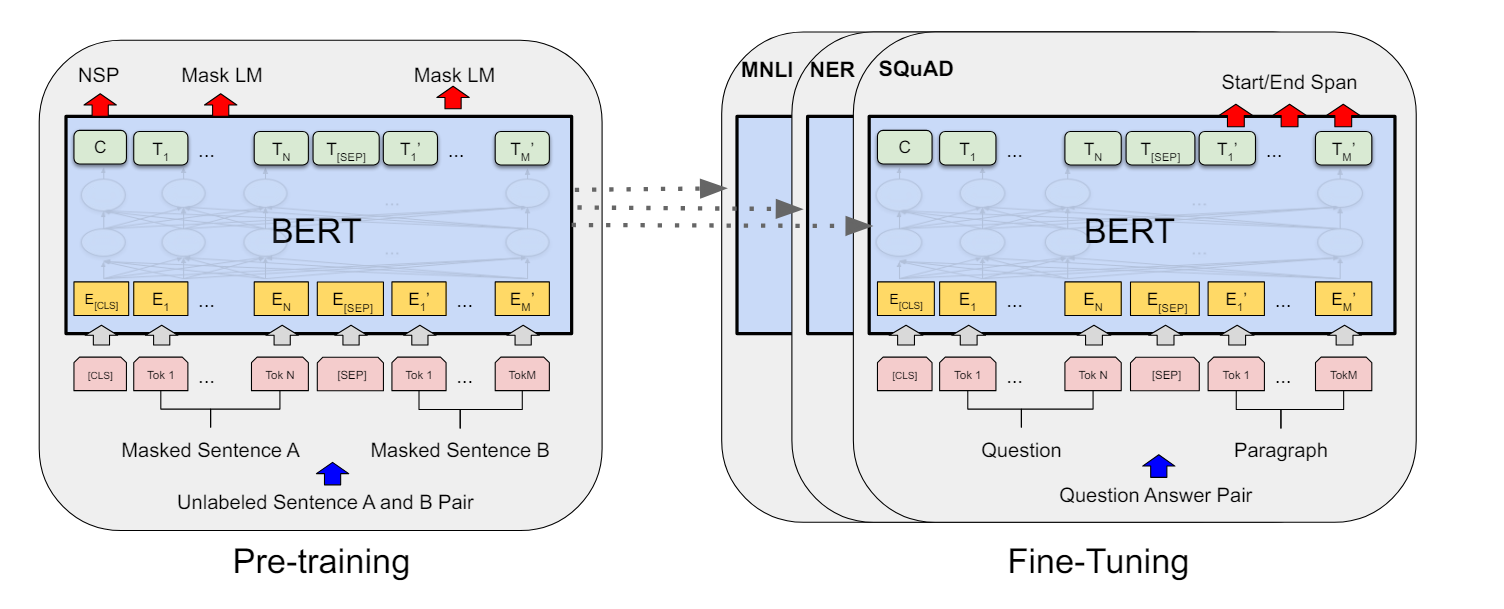
\includegraphics[width=0.8\textwidth]{BERT Finetuning.png}
  \caption{Finetuning in the BERT model \cite{Devlin18}}
  \label{fig:bert_finetune}
\end{figure}

\section{Conclusion}
In this section, I will shortly summarize the outline of this paper and also talk about the possible future development of large language models using data streams.

%\paragraph{Sample Heading (Fourth Level)}
%The contribution should contain no more than four levels of
%headings. Table~\ref{tab1} gives a summary of all heading levels.
\begin{comment}
\begin{table}
\caption{Table captions should be placed above the
tables.}\label{tab1}
\begin{tabular}{|l|l|l|}
\hline
Heading level &  Example & Font size and style\\
\hline
Title (centered) &  {\Large\bfseries Lecture Notes} & 14 point, bold\\
1st-level heading &  {\large\bfseries 1 Introduction} & 12 point, bold\\
2nd-level heading & {\bfseries 2.1 Printing Area} & 10 point, bold\\
3rd-level heading & {\bfseries Run-in Heading in Bold.} Text follows & 10 point, bold\\
4th-level heading & {\itshape Lowest Level Heading.} Text follows & 10 point, italic\\
\hline
\end{tabular}
\end{table}


\noindent Displayed equations are centered and set on a separate
line.
\begin{equation}
x + y = z
\end{equation}
Please try to avoid rasterized images for line-art diagrams and
schemas. Whenever possible, use vector graphics instead (see
Fig.~\ref{fig1}).

\begin{figure}
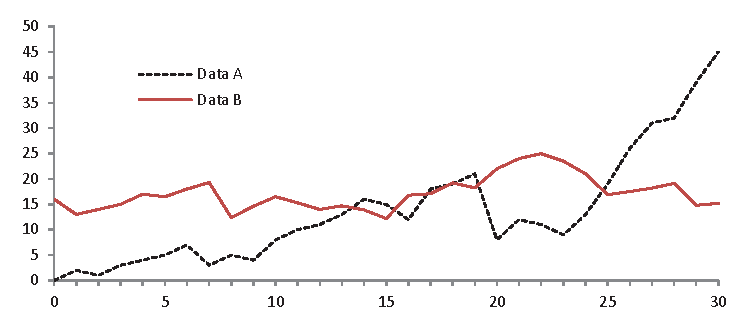
\includegraphics[width=\textwidth]{fig1.eps}
\caption{A figure caption is always placed below the illustration.
Please note that short captions are centered, while long ones are
justified by the macro package automatically.} \label{fig1}
\end{figure}

\begin{theorem}
This is a sample theorem. The run-in heading is set in bold, while
the following text appears in italics. Definitions, lemmas,
propositions, and corollaries are styled the same way.
\end{theorem}
%
% the environments 'definition', 'lemma', 'proposition', 'corollary',
% 'remark', and 'example' are defined in the LLNCS documentclass as well.
%
\begin{proof}
Proofs, examples, and remarks have the initial word in italics,
while the following text appears in normal font.
\end{proof}
For citations of references, we prefer the use of square brackets
and consecutive numbers. Citations using labels or the author/year
convention are also acceptable. The following bibliography provides
a sample reference list with entries for journal
articles~\cite{ref_article1}, an LNCS chapter~\cite{ref_lncs1}, a
book~\cite{ref_book1}, proceedings without editors~\cite{ref_proc1},
and a homepage~\cite{ref_url1}. Multiple citations are grouped
\cite{ref_article1,ref_lncs1,ref_book1},
\cite{ref_article1,ref_book1,ref_proc1,ref_url1}.

\begin{credits}
\subsubsection{\ackname} A bold run-in heading in small font size at the end of the paper is
used for general acknowledgments, for example: This study was funded
by X (grant number Y).

\subsubsection{\discintname}
It is now necessary to declare any competing interests or to specifically
state that the authors have no competing interests. Please place the
statement with a bold run-in heading in small font size beneath the
(optional) acknowledgments\footnote{If EquinOCS, our proceedings submission
system, is used, then the disclaimer can be provided directly in the system.},
for example: The authors have no competing interests to declare that are
relevant to the content of this article. Or: Author A has received research
grants from Company W. Author B has received a speaker honorarium from
Company X and owns stock in Company Y. Author C is a member of committee Z.
\end{credits}
\end{comment}
%
% ---- Bibliography ----
%
% BibTeX users should specify bibliography style 'splncs04'.
% References will then be sorted and formatted in the correct style.
%
\bibliographystyle{splncs04}
%\bibliography{LLMs and Data Streams}
%

\begin{thebibliography}{8}
\begin{comment}
\bibitem{ref_article1}
Author, F.: Article title. Journal \textbf{2}(5), 99--110 (2016)

\bibitem{ref_lncs1}
Author, F., Author, S.: Title of a proceedings paper. In: Editor,
F., Editor, S. (eds.) CONFERENCE 2016, LNCS, vol. 9999, pp. 1--13.
Springer, Heidelberg (2016). \doi{10.10007/1234567890             }

\bibitem{ref_book1}
Author, F., Author, S., Author, T.: Book title. 2nd edn. Publisher,
Location (1999)

\bibitem{ref_proc1}
Author, A.-B.: Contribution title. In: 9th International Proceedings
on Proceedings, pp. 1--2. Publisher, Location (2010)

\bibitem{ref_url1}
LNCS Homepage, \url{http://www.springer.com/lncs}, last accessed 2023/10/25
\end{comment}
\bibitem{Liu23}
Liu, Yiheng, Tianle Han, Siyuan Ma, Jiayue Zhang, Yuanyuan Yang, Jiaming Tian, Hao He et al. "Summary of chatgpt-related research and perspective towards the future of large language models." Meta-Radiology (2023): 100017.

\bibitem{Kasneci23}
Kasneci, Enkelejda, Kathrin Seßler, Stefan Küchemann, Maria Bannert, Daryna Dementieva, Frank Fischer, Urs Gasser et al. "ChatGPT for good? On opportunities and challenges of large language models for education." Learning and individual differences 103 (2023): 102274.

\bibitem{Thiru23}
Thirunavukarasu, Arun James, Darren Shu Jeng Ting, Kabilan Elangovan, Laura Gutierrez, Ting Fang Tan, and Daniel Shu Wei Ting. "Large language models in medicine." Nature medicine 29, no. 8 (2023): 1930-1940.

\bibitem{Chang23}
Chang, Yupeng, Xu Wang, Jindong Wang, Yuan Wu, Linyi Yang, Kaijie Zhu, Hao Chen et al. "A survey on evaluation of large language models." ACM Transactions on Intelligent Systems and Technology (2023).

\bibitem{Zhang23}
Zhang, Shuhao, Xianzhi Zeng, Yuhao Wu, and Zhonghao Yang. "Harnessing scalable transactional stream processing for managing large language models [vision]." arXiv preprint arXiv:2307.08225 (2023).

\bibitem{Zhang24}
Zhang, Kunpeng, Feng Zhou, Lan Wu, Na Xie, and Zhengbing He. "Semantic understanding and prompt engineering for large-scale traffic data imputation." Information Fusion 102 (2024): 102038.

\bibitem{Xu23}
Xu, Xuhai, Bingshen Yao, Yuanzhe Dong, Hong Yu, James Hendler, Anind K. Dey, and Dakuo Wang. "Leveraging large language models for mental health prediction via online text data." arXiv preprint arXiv:2307.14385 (2023).

\bibitem{Zhang_Xin24}
Zhang, Xin, Linhai Zhang, Deyu Zhou, and Guoqiang Xu. "Fine-grainedly Synthesize Streaming Data Based On Large Language Models With Graph Structure Understanding For Data Sparsity." arXiv preprint arXiv:2403.06139 (2024).

\bibitem{Wu24}
Wu, Tongtong, Linhao Luo, Yuan-Fang Li, Shirui Pan, Thuy-Trang Vu, and Gholamreza Haffari. "Continual learning for large language models: A survey." arXiv preprint arXiv:2402.01364 (2024).

\bibitem{Brown20}
Brown, Tom, Benjamin Mann, Nick Ryder, Melanie Subbiah, Jared D. Kaplan, Prafulla Dhariwal, Arvind Neelakantan et al. "Language models are few-shot learners." Advances in neural information processing systems 33 (2020): 1877-1901.

\bibitem{Gama13}
Gama, Joao, Raquel Sebastiao, and Pedro Pereira Rodrigues. "On evaluating stream learning algorithms." Machine learning 90 (2013): 317-346.

\bibitem{Jang21}
Jang, Joel, Seonghyeon Ye, Sohee Yang, Joongbo Shin, Janghoon Han, Gyeonghun Kim, Stanley Jungkyu Choi, and Minjoon Seo. "Towards continual knowledge learning of language models." arXiv preprint arXiv:2110.03215 (2021).

\bibitem{Geisler13}
Geisler, Sandra. "Data stream management systems." In Dagstuhl Follow-Ups, vol. 5. Schloss Dagstuhl-Leibniz-Zentrum fuer Informatik, 2013.

\bibitem{Geisler16}
Geisler, Sandra. "A systematic evaluation approach for data stream-based applications." PhD diss., Dissertation, RWTH Aachen University, 2016, 2016.

\bibitem{Vaswani17}
Vaswani, Ashish, Noam Shazeer, Niki Parmar, Jakob Uszkoreit, Llion Jones, Aidan N. Gomez, Łukasz Kaiser, and Illia Polosukhin. "Attention is all you need." Advances in neural information processing systems 30 (2017).

\bibitem{Devlin18}
Devlin, Jacob, Ming-Wei Chang, Kenton Lee, and Kristina Toutanova. "Bert: Pre-training of deep bidirectional transformers for language understanding." arXiv preprint arXiv:1810.04805 (2018).

\bibitem{Yenduri24}
Yenduri, Gokul, M. Ramalingam, G. Chemmalar Selvi, Y. Supriya, Gautam Srivastava, Praveen Kumar Reddy Maddikunta, G. Deepti Raj et al. "GPT (Generative Pre-trained Transformer)–A Comprehensive Review on Enabling Technologies, Potential Applications, Emerging Challenges, and Future Directions." IEEE Access (2024).

\bibitem{Lester21}
Lester, Brian, Rami Al-Rfou, and Noah Constant. "The power of scale for parameter-efficient prompt tuning." arXiv preprint arXiv:2104.08691 (2021).

\bibitem{So19}
So, David, Quoc Le, and Chen Liang. "The evolved transformer." In International conference on machine learning, pp. 5877-5886. PMLR, 2019.

\bibitem{Zhao22}
Zhao, Feng, Xinning Li, Yating Gao, Ying Li, Zhiquan Feng, and Caiming Zhang. "Multi-layer features ablation of BERT model and its application in stock trend prediction." Expert Systems with Applications 207 (2022): 117958.

\bibitem{Ren24}
Ren, Yilong, Yue Chen, Shuai Liu, Boyue Wang, Haiyang Yu, and Zhiyong Cui. "TPLLM: A Traffic Prediction Framework Based on Pretrained Large Language Models." arXiv preprint arXiv:2403.02221 (2024).

\bibitem{Liu24}
Liu, Chenxi, Sun Yang, Qianxiong Xu, Zhishuai Li, Cheng Long, Ziyue Li, and Rui Zhao. "Spatial-temporal large language model for traffic prediction." arXiv preprint arXiv:2401.10134 (2024).

\bibitem{Yang22}
Yang, Xi, Aokun Chen, Nima PourNejatian, Hoo Chang Shin, Kaleb E. Smith, Christopher Parisien, Colin Compas et al. "A large language model for electronic health records." NPJ digital medicine 5, no. 1 (2022): 194.

\bibitem{Gupta23}
Gupta, Kshitij, Benjamin Thérien, Adam Ibrahim, Mats L. Richter, Quentin Anthony, Eugene Belilovsky, Irina Rish, and Timothée Lesort. "Continual Pre-Training of Large Language Models: How to (re) warm your model?." arXiv preprint arXiv:2308.04014 (2023).

\bibitem{Naga23}
Naga Sanjay, "Continuous Training of ML models. A case-study on how to keep our machine learning models relevant.", Medium, June 25, 2023

\bibitem{Prapas21}
Prapas, Ioannis, Behrouz Derakhshan, Alireza Rezaei Mahdiraji, and Volker Markl. "Continuous training and deployment of deep learning models." Datenbank-Spektrum 21, no. 3 (2021): 203-212.

\bibitem{Araci19}
Araci, Dogu. "Finbert: Financial sentiment analysis with pre-trained language models." arXiv preprint arXiv:1908.10063 (2019).

\bibitem{Roum23}
Roumeliotis, Konstantinos I., and Nikolaos D. Tselikas. "Chatgpt and open-ai models: A preliminary review." Future Internet 15, no. 6 (2023): 192.

\bibitem{Cavnar94}
Cavnar, William B., and John M. Trenkle. "N-gram-based text categorization." In Proceedings of SDAIR-94, 3rd annual symposium on document analysis and information retrieval, vol. 161175, p. 14. 1994.

\bibitem{Mikolov13}
Mikolov, Tomas, Ilya Sutskever, Kai Chen, Greg S. Corrado, and Jeff Dean. "Distributed representations of words and phrases and their compositionality." Advances in neural information processing systems 26 (2013).

\bibitem{Sutskever14}
Sutskever, Ilya, Oriol Vinyals, and Quoc V. Le. "Sequence to sequence learning with neural networks." Advances in neural information processing systems 27 (2014).

\bibitem{Radford19}
Radford, Alec, Jeffrey Wu, Rewon Child, David Luan, Dario Amodei, and Ilya Sutskever. "Language models are unsupervised multitask learners." OpenAI blog 1, no. 8 (2019): 9.

\bibitem{Radford18}
Radford, Alec, Karthik Narasimhan, Tim Salimans, and Ilya Sutskever. "Improving language understanding by generative pre-training." (2018).

\bibitem{Kaplan20}
Kaplan, Jared, Sam McCandlish, Tom Henighan, Tom B. Brown, Benjamin Chess, Rewon Child, Scott Gray, Alec Radford, Jeffrey Wu, and Dario Amodei. "Scaling laws for neural language models." arXiv preprint arXiv:2001.08361 (2020).

\bibitem{Gozalo23}
Gozalo-Brizuela, Roberto, and Eduardo C. Garrido-Merchan. "ChatGPT is not all you need. A State of the Art Review of large Generative AI models." arXiv preprint arXiv:2301.04655 (2023).

\bibitem{Patro06}
Patroumpas, Kostas, and Timos Sellis. "Window specification over data streams." In International Conference on Extending Database Technology, pp. 445-464. Berlin, Heidelberg: Springer Berlin Heidelberg, 2006.

\bibitem{Golab03}
Golab, Lukasz, and M. Tamer Özsu. "Issues in data stream management." ACM Sigmod Record 32, no. 2 (2003): 5-14.

\bibitem{Gaber05}
Gaber, Mohamed Medhat, Arkady Zaslavsky, and Shonali Krishnaswamy. "Mining data streams: a review." ACM Sigmod Record 34, no. 2 (2005): 18-26.
\end{thebibliography}

\end{document}
